\def\uRadius{(0, 0) circle (1.5cm)}
\def\vRadius{(1.5, 0) circle (1.5cm)}

\def\ggRadius{(0.75, 0) circle(0.75cm)}

\colorlet{circle edge}{black!50}
\colorlet{circle area}{gray!20}

\tikzset{
  filled/.style={fill=circle area, draw=circle edge, thick},
  outline/.style={draw=circle edge, thick}
  }

\setlength{\parskip}{5mm}

\tikzstyle{edge} = [draw, thick,-]
\tikzstyle{vertex}=[circle,fill=black!25,minimum size=10pt,inner sep=0pt]
\tikzstyle{invis-vertex}=[circle,fill=white!100,minimum size=0pt, inner sep=0pt]

\subfloat[No node in intersection]{\label{fig:rng1}
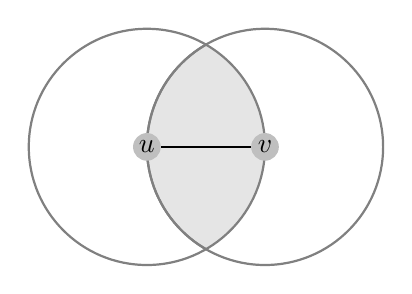
\begin{tikzpicture} 
   
  \begin{scope}
    \clip \uRadius;
    \fill[filled] \vRadius;
  \end{scope}

  \draw[outline] \uRadius node {};
  \draw[outline] \vRadius node {};

  \foreach \pos/\name in {{(0, 0)/u}, {(1.5, 0)/v}} {
    \node[vertex] (\name) at \pos {$\name$};
  }

  \path[edge] (u) -- (v);
\end{tikzpicture}}
% Remove empty line
\subfloat[A node in the intersection]{\label{fig:rng2}
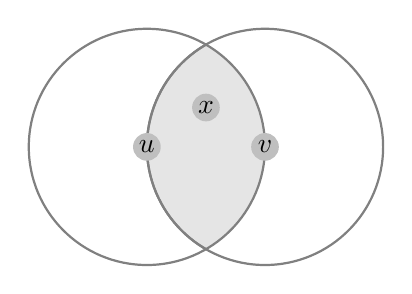
\begin{tikzpicture} 
   
  \begin{scope}
    \clip \uRadius;
    \fill[filled] \vRadius;
  \end{scope}

  \draw[outline] \uRadius node {};
  \draw[outline] \vRadius node {};

  \foreach \pos/\name in {{(0, 0)/u}, {(1.5, 0)/v}, {(0.75, 0.5)/x}} {
    \node[vertex] (\name) at \pos {$\name$};
  }

\end{tikzpicture}}

\subfloat[No node in the diameter circle]{\label{fig:gabe1}
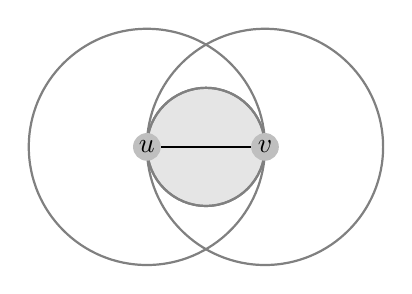
\begin{tikzpicture}    
  \begin{scope}
    \fill[filled] \ggRadius;
  \end{scope}

  \draw[outline] \uRadius node {};
  \draw[outline] \vRadius node {};
  \draw[outline] \ggRadius node {};

  \foreach \pos/\name in {{(0, 0)/u}, {(1.5, 0)/v}} {
    \node[vertex] (\name) at \pos {$\name$};
  }

  \path[edge] (u) -- (v);
\end{tikzpicture}}
%remove empty line
\subfloat[A node in the diameter circle]{\label{fig:gabe2}
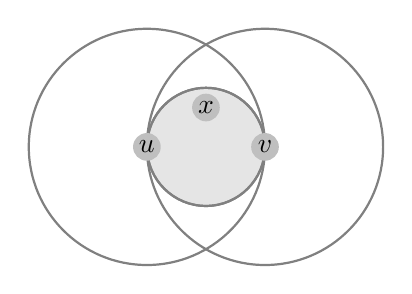
\begin{tikzpicture}    
  \begin{scope}
    \fill[filled] \ggRadius;
  \end{scope}

  \draw[outline] \uRadius node {};
  \draw[outline] \vRadius node {};
  \draw[outline] \ggRadius node {};

  \foreach \pos/\name in {{(0, 0)/u}, {(1.5, 0)/v}, {(0.75, 0.5)/x}} {
    \node[vertex] (\name) at \pos {$\name$};
  }
\end{tikzpicture}}
